\documentclass{article}
\usepackage[utf8]{inputenc}
\usepackage{listings}
\usepackage{graphicx}
\usepackage{float}
\usepackage{xcolor}
\usepackage{geometry}
\usepackage{CJKutf8}
\usepackage{amsmath}
\usepackage{amssymb}

\geometry{a4paper,scale=0.8}
\lstset{
    basicstyle          =   \sffamily,        
    keywordstyle        =   \bfseries,         
    commentstyle        =   \rmfamily\itshape, 
    stringstyle         =   \ttfamily, 
    flexiblecolumns,               
    numbers             =   left,  
    showspaces          =   false, 
    showstringspaces    =   false,
    captionpos          =   t,     
    frame               =   lrtb, 
}

\lstdefinestyle{Python}{
    language        =   Python, % 语言选Python
    basicstyle      =   \zihao{-5}\ttfamily,
    numberstyle     =   \zihao{-5}\ttfamily,
    keywordstyle    =   \color{blue},
    keywordstyle    =   [2] \color{teal},
    stringstyle     =   \color{magenta},
    commentstyle    =   \color{red}\ttfamily,
    breaklines      =   true,  
    columns         =   fixed,  
    basewidth       =   0.5em,
}

\title{\bf\Large  概率论与数理统计 第12次作业}
%%%%%%%%%%%%%%%%%%%%%%%%%%%%%%%%%%%%%%
%% DON'T forget to change this part %%
\author{\bf Name: 宋昊原 \qquad Student ID: 2022010755}
%%%%%%%%%%%%%%%%%%%%%%%%%%%%%%%%%%%%%%

\begin{document}
\begin{CJK}{UTF8}{gbsn}
\maketitle
\section{指数分布假设检验}
\subsection{双边检验}
设
$$ H_{0}:\ \lambda = \lambda_{0} $$
$$ H_{1}:\ \lambda \neq \lambda_{0} $$
规定拒绝域的形状为
$$ \vert\bar{X}-\frac{1}{\lambda_{0}}\vert\geq c$$
根据中心极限定理,当$n$很大时,近似地有
$$ \frac{\bar{X}-\frac{1}{\lambda_{0}}}{\frac{1}{\lambda_{0}\sqrt{n}}}\sim {\rm N}(0,1)$$
于是,只需取
$$ c = \frac{1}{\lambda_{0}\sqrt{n}}Z_{\frac{\alpha}{2}}$$
其中$Z_{x}$表示标准正态的上$x$分位数
\\\\故显著性水平为$\alpha$时,如果
$$ \vert\bar{X}-\frac{1}{\lambda_{0}}\vert < \frac{1}{\lambda_{0}\sqrt{n}}Z_{\frac{\alpha}{2}}$$
则不拒绝$H_{0}$,否则拒绝之.
\subsection{单边检验}
设
$$ H_{0}:\ \lambda \leq \lambda_{0} $$
$$ H_{1}:\ \lambda > \lambda_{0} $$
规定拒绝域的形状为
$$ \bar{X}\leq c$$
根据中心极限定理,当$n$很大时,近似地有
$$ \frac{\bar{X}-\frac{1}{\lambda_{0}}}{\frac{1}{\lambda_{0}\sqrt{n}}}\sim {\rm N}(0,1)$$
于是,只需取
$$ c = \frac{1}{\lambda_{0}}-\frac{1}{\lambda_{0}\sqrt{n}}Z_{\alpha}$$
故显著性水平为$\alpha$时,如果
$$ \bar{X}\geq\frac{1}{\lambda_{0}}-\frac{1}{\lambda_{0}\sqrt{n}}Z_{\alpha}$$
则不拒绝$H_{0}$.
\section{均匀分布的假设检验}
\subsection{利用矩估计量}
矩估计为
$$ \theta = 2\bar{X}$$
故拒绝域应为
$$ \bar{X} \geq c $$
根据中心极限定理,当$n$很大时,近似地有
$$ \frac{\bar{X}-\frac{\theta}{2}}{\frac{\theta}{\sqrt{12n}}}\sim {\rm N}(0,1)$$
于是
$$ c = \frac{\theta_{0}}{2} + \frac{\theta_{0}}{\sqrt{12n}}Z_{\alpha} $$
下面计算其功效
$$ 1-\beta(R)={\rm P}_{\theta>\theta_{0}}(R)=\frac{\theta-\theta_{0}(\frac{1}{2}+\frac{Z_{\alpha}}{\sqrt{12n}})}{\theta}=1-\frac{\theta_{0}}{\theta}(\frac{1}{2}+\frac{Z_{\alpha}}{\sqrt{12n}})$$
\subsection{利用极大似然估计量}
极大似然估计为
$$ \theta^{*}=\max\{X_{1},...,X_{n}\}=:X_{M}$$
拒绝域为
$$ X_{M}\geq c $$
且满足
$$ {\rm P}_{\theta_{0}}(X_{M}\geq c)=\alpha $$
由于$X_{M}$的CDF为
$$ F_{n}(x)=(\frac{x}{\theta})^{n}$$
故
$$ 1-(\frac{c}{\theta_{0}})^{n}=\alpha$$
$$ c = \theta_{0}(1-\alpha)^{\frac{1}{n}}$$
下面计算其功效
$$ 1-\beta(R)={\rm P}_{\theta>\theta_{0}}(R)=1-(\frac{c}{\theta})^{n}=1-(1-\alpha)(\frac{\theta_{0}}{\theta})^{n}$$
\section{高危职业}
设该公司雇员病假天数总体为$X\sim {\rm N}(\mu,\sigma^{2})$,现构造以下假设检验:
$$ H_{0}:\ \mu=\mu_{0}$$
$$ H_{1}:\ \mu>\mu_{0}$$
其中
$$ \mu_{0} = 5.1 $$
$$ \mu = 7 $$
$$ \sigma = 2.5 $$
$$ n = 49 $$
现规定显著性水平
$$ \alpha = 0.05 $$
拒绝域形式为
$$ \bar{X}\geq c $$
由于
$$ \bar{X}\sim{\rm N}(\mu,\frac{\sigma^{2}}{n})$$
有
$$ c = \mu_{0} + \frac{\sigma}{\sqrt{n}}Z_{\alpha} $$
计算得
$$ c = 5.687 $$
故在$\alpha=0.05$的显著性水平下可以拒绝$H_{0}$,该公司员工比常人更容易生病.\ 事实上即使显著性水平降至0.01,仍有充分的理由拒绝$H_{0}$.
\section{灯泡合格}
\subsection{}
设寿命总体$X\sim{\rm N}(\mu,\sigma^{2})$,$\mu_{0}=1180$,则
$$ H_{0}:\ \mu\geq\mu_{0}$$
$$ H_{1}:\ \mu<\mu_{0}$$
设拒绝域形式为
$$ \bar{X}\leq c$$
由于
$$ \frac{\bar{X}-\mu}{S/\sqrt{n}}\sim{\rm t}(n-1)$$
有
$$ c=\mu_{0} - \frac{S}{\sqrt{n}}t_{\alpha}$$
以$\alpha = 0.05$为显著性水平,计算得
$$ c=1084.9$$
而
$$\bar{X}=1160$$
故在0.05显著性水平下,不能拒绝$H_{0}$,灯泡合格.
\subsection{}
互换原假设和备择假设,拒绝域形式将变为
$$ X\geq c$$
而
$$ c=\mu_{0} + \frac{S}{\sqrt{n}}t_{\alpha}$$
此时
$$ c = 1275.1 $$
故在0.05显著性水平下,也不能拒绝$H_{1}$(此时仍用$H_{1}$表示新的原假设),也不能拒绝灯泡不合格的假设.
\\\\
这是因为这些灯泡寿命的均值与临界值1180较接近,同时其样本标准差较大,因此两种原假设的拒绝域都很极端,非拒绝域则有很大的重叠,因此两种假设都不能拒绝.
\subsection{}
假设选择$\alpha = 0.95$,这实际上与之前得到完全相反的结论,即
$$ \bar{X}\leq 1275.1 $$时拒绝$H_{0}$,
$$ \bar{X}\geq 1084.9 $$时拒绝$H_{1}$.
\\\\
这导致两种假设实际上都被拒绝.
\section{元件寿命}
$$ H_{0}:\ \mu\leq\mu_{0}$$
$$ H_{1}:\ \mu>\mu_{0}$$
拒绝域为
$$ \bar{X}\geq c$$
其中
$$ c = \mu_{0}+\frac{S}{\sqrt{n}}t_{\alpha}$$
计算得
$$ c = 268.27$$
$$ \bar{X}=241.5 $$
故没有理由拒绝$H_{0}$,即没有充分的理由认为$\mu>225$.
\section{Poisson分布大样本检验}
当$n$很大时,近似地有
$$ \bar{X}\sim{\rm N}(\lambda,\frac{\lambda}{n})$$
于是,拒绝域形式为
$$ \vert\bar{X}-\lambda_{0}\vert\geq c$$
其中
$$ c = \sqrt{\frac{\lambda_{0}}{n}}Z_{\frac{\alpha}{2}}$$
\section{错误比例}
\subsection{}
原假设为真的情况下第一类错误的比例为
$$\frac{200}{4000}=\frac{1}{20}$$
\subsection{}
拒绝了原假设的情况下第一类错误的比例为
$$\frac{200}{700}=\frac{2}{7}$$
显著性水平为0.05并不代表平均每20次拒绝原假设只有1次发生错误.
\subsection{}
原假设为假的情况下第二类错误的比例为
$$\frac{500}{1000}=\frac{1}{2}$$
\subsection{}
检验的功效为
$$ 1-\beta = \frac{1}{2}$$
\section{治愈癌症}
\subsection{}
上述判断不科学,应使用假设检验的方法.
\\\\设化学疗法总体符合Bernoulli分布${\rm B}(p)$,$p_{0}=0.02$,设
$$ H_{0}:\ p \leq p_{0}$$
$$ H_{1}:\ p > p_{0}$$
拒绝域形式为
$$ \bar{X}\geq c $$
由于
$$ n\bar{X}\sim{\rm B}(n,p)$$
令显著性水平$\alpha=0.05$,只需要找到二项分布${\rm B}(n,p_{0})$的上$\alpha$分位数,并与$n\bar{X}$比较即可.
\subsection{}
代入数据,计算机计算得,$\alpha=0.05$对应的拒绝域为
$$ n\bar{X}\geq 8 $$
而
$$ n\bar{X}=6 $$
故没有理由拒绝$H_{0}$,不能说明化学疗法比外科疗法治愈率高.
\section{计算机实验:Poisson分布的假设检验}
\begin{minipage}{0.5\textwidth}
    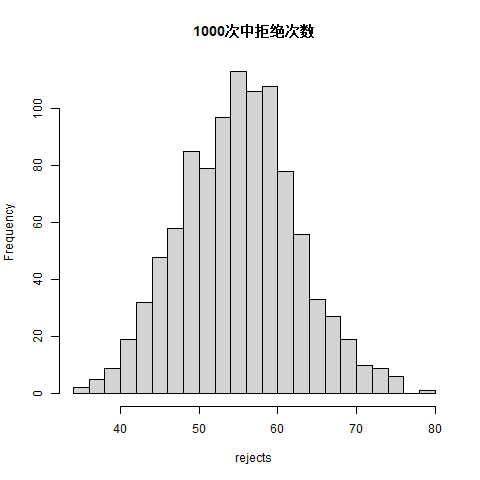
\includegraphics[scale=0.6]{poisson_check.png}
\end{minipage}
\\
可见,拒绝次数比较接近50,但实际集中在比50略高一些位置,这可能是由于$n=20$时中心极限定理的近似不是很好导致的.
\\\\
当我将$n=20$改为$n=1000$时,拒绝次数的均值、中位数都更接近50.\\
\begin{minipage}{0.5\textwidth}
    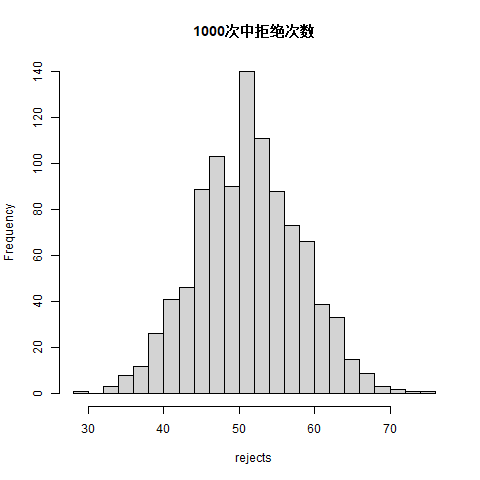
\includegraphics[scale=0.6]{poisson_check_big.png}
\end{minipage}
\end{CJK}
\end{document}